% Created 2021-03-04 Thu 05:30
% Intended LaTeX compiler: pdflatex
\documentclass[presentation]{beamer}
\usepackage[utf8]{inputenc}
\usepackage[T1]{fontenc}
\usepackage{graphicx}
\usepackage{grffile}
\usepackage{longtable}
\usepackage{wrapfig}
\usepackage{rotating}
\usepackage[normalem]{ulem}
\usepackage{amsmath}
\usepackage{textcomp}
\usepackage{amssymb}
\usepackage{capt-of}
\usepackage{hyperref}
\usetheme{metropolis}
\usecolortheme{}
\usefonttheme{}
\useinnertheme{}
\useoutertheme{}
\author{Petru Rebeja, Marius Apetrii}
\date{25 Februarie 2021}
\title{Tehnici Avansate de Programare}
\subtitle{Recapitulare și noțiuni de bază}
\institute[UAIC]{Facultatea de Matematică\\Universitatea Alexandru Ioan Cuza, Iași}
\hypersetup{
 pdfauthor={Petru Rebeja, Marius Apetrii},
 pdftitle={Tehnici Avansate de Programare},
 pdfkeywords={},
 pdfsubject={},
 pdfcreator={Emacs 26.3 (Org mode 9.4.4)},
 pdflang={Romanian}}
\begin{document}

\maketitle
\section{Introducere}
\label{sec:orgdc78b31}
\begin{frame}[label={sec:orga7ba789}]{Ce am discutat data trecută}
\pause
\begin{itemize}
\item Ciclul de dezvoltare al aplicațiilor
\item Dezvoltarea în iterații
\item Unelte de lucru
\item Fluxul de lucru Git
\item Bune practici
\end{itemize}
\end{frame}
\begin{frame}[label={sec:org364043d},fragile]{Ce vom discuta azi}
 \begin{itemize}
\item Tipuri de date în \texttt{.net}
\item Principiile programării orientată-obiect
\end{itemize}
\end{frame}
\section{Tipuri de date în \texttt{.net}}
\label{sec:org0646ae4}
\begin{frame}[label={sec:orgfc5367a},fragile]{Tipuri \texttt{referință} și tipuri \texttt{valoare}}
 \begin{center}
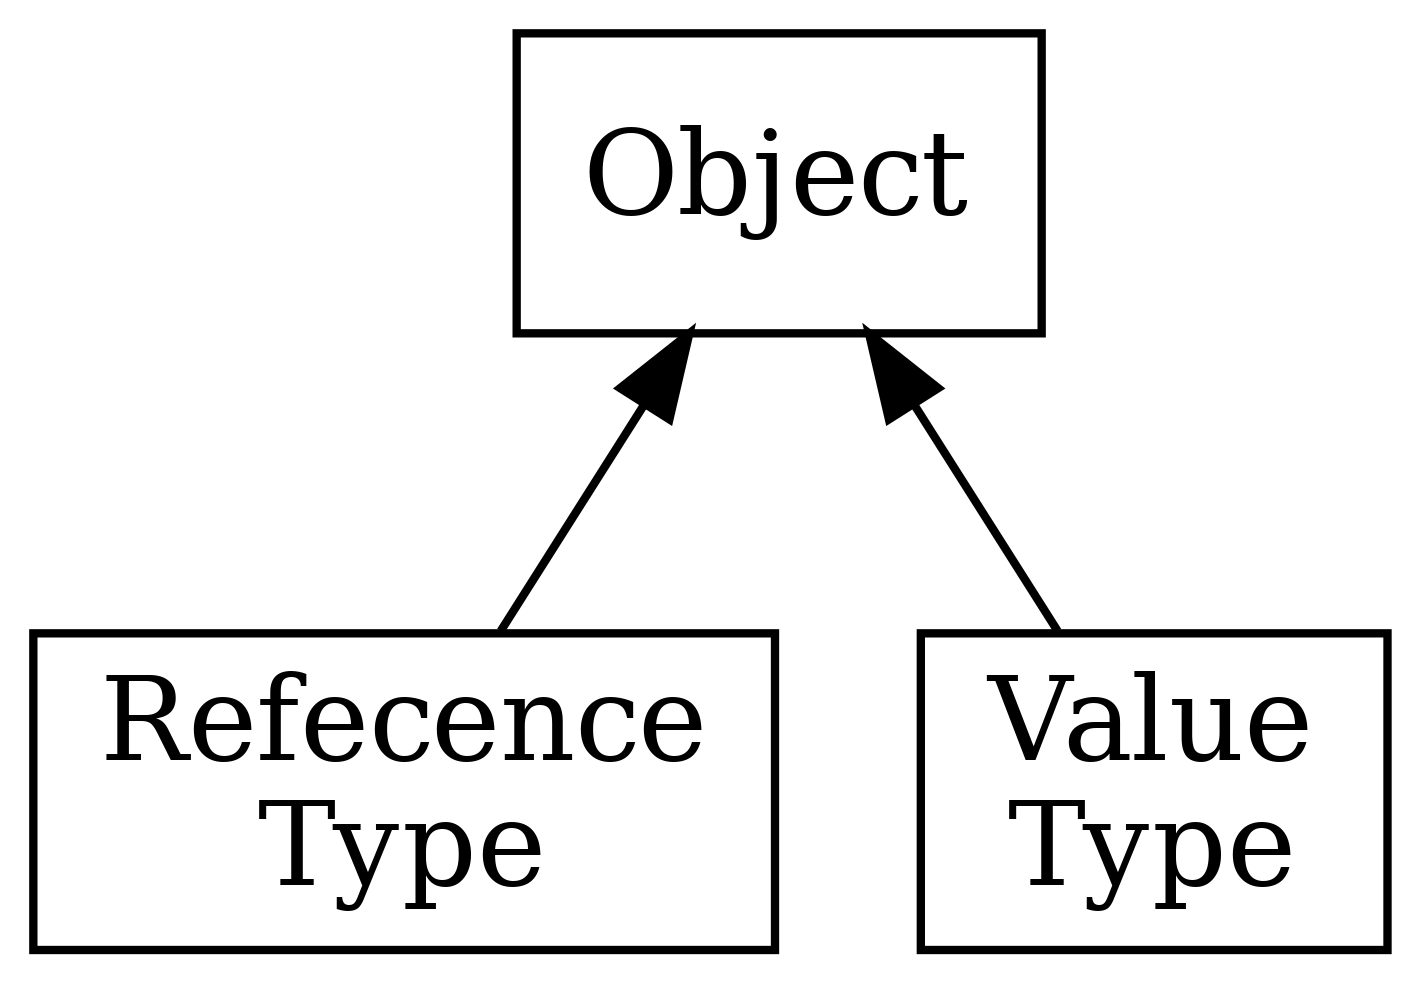
\includegraphics[width=0.6\textwidth]{./img/netcore-types.png}
\end{center}
\end{frame}
\begin{frame}[label={sec:org60b6bd6},fragile]{Tipuri \texttt{referință} și tipuri \texttt{valoare}}
 \begin{block}{Exemple}
\begin{center}
\begin{tabular}{ll}
Tip Referință & Tip Valoare\\
\hline
\texttt{string} & \texttt{int}\\
\texttt{System.Object} & \texttt{float}\\
\texttt{System.Action} & \texttt{bool}\\
\texttt{System.IO.MemoryStream} & Tipuri \texttt{struct}\\
\texttt{System.Collections.Generic.List<T>} & Tipuri \texttt{enum}\\
\end{tabular}
\end{center}
\end{block}
\end{frame}
\begin{frame}[label={sec:orgb6bcafd},fragile]{Tipuri \texttt{valoare}}
 \begin{itemize}
\item O variabilă a unui tip valoare conține o instanță a tipului respectiv.
\item La crearea unei instanțe se alocă o singură zonă în memorie.
\item Dimensiunea zonei alocate este dată de tip.
\end{itemize}
\end{frame}
\begin{frame}[label={sec:orgd679509},fragile]{Tipuri \texttt{referință}}
 \begin{itemize}
\item O variabilă a unui tip referință conține adresa de memorie unde este alocată instanța propriu-zisă.
\item La crearea unei instanțe se alocă două zone de memorie:
\begin{itemize}
\item O zonă pentru adresă (stivă),
\item O zonă pentru instanță (memoria heap).
\end{itemize}
\item Dimensiunea zonei alocate pentru instanță poate să varieze (ex. \texttt{List<T>}).
\end{itemize}
\end{frame}
\begin{frame}[label={sec:org8d3a5e9},fragile]{Cazul special: \texttt{string}}
 \begin{itemize}
\item Deși tipul \texttt{string} este un tip referință, acesta se comportă ca un tip valoare.
\item Această proprietate se numește \texttt{imuabilitate}
\end{itemize}
\end{frame}
\section{Principiile Programării Orientate-Obiect}
\label{sec:orge64a4fa}
\begin{frame}[label={sec:org06a2f72}]{Recapitulare}
\begin{itemize}
\item \alert{Încapsularea} --- îmbinarea datelor și metodelor care le procesează.
\item \alert{Moștenire} --- proprietățile tipului părinte se păstrează și la copii.
\item \alert{Polimorfism} --- același comportament manifestat de mai multe tipuri.
\end{itemize}
\end{frame}
\begin{frame}[label={sec:org47871e6}]{Exemplificare}
\begin{block}{Context}
\vskip 0.1in
Pentru exemplificare vom modela o serie de operațiuni bancare.
\end{block}
\end{frame}
\begin{frame}[label={sec:org29d3b71}]{Exemplificare}
\begin{block}{Cerință I}
\vskip 0.1in
În calitate de posesor al unui cont bancar vreau să pot depune și extrage diverse sume de bani din cont.
\end{block}
\end{frame}
\begin{frame}[label={sec:org9586615}]{Încapsularea}
În situația de față, \alert{încapsularea} ne permite să îmbinăm retragerea de fonduri cu verificarea dacă sunt fonduri suficiente.
\end{frame}
\begin{frame}[label={sec:orgb045d57}]{Exemplificare}
\begin{block}{Cerință II}
\vskip 0.1in
În calitate de posesor de conturi, pot avea conturi de diferite tipuri: economii și debit. Pentru retragerea de fonduri din fiecare cont se percep comisioane diferite în funcție de tipul acestuia:
\begin{itemize}
\item Pentru contul de debit: 0 \%
\item Pentru contul de economii: 0.5 \%
\end{itemize}
\end{block}
\end{frame}
\begin{frame}[label={sec:org4533038}]{Exemplificare}
\begin{block}{Cerință III}
\vskip 0.1in
În calitate de posesor de conturi pot avea un cont de credit cu un comision de retragere de 0.7\%
\end{block}
\end{frame}
\begin{frame}[label={sec:org0f0cf3f}]{Moștenirea}
În exemplul dat \alert{moștenirea} ne permite să declarăm o clasă de bază cu proprietățile comune și să implementăm particularitățile în clasele derivate.
\end{frame}
\begin{frame}[label={sec:orgf9e6a6e}]{Polimorfismul}
\alert{Polimorfismul} ne permite să aplicăm reguli de calcul diferite pentru aceeași metodă.
\end{frame}
\section{Încheiere}
\label{sec:org5b4f986}
\begin{frame}[label={sec:org59050df},fragile]{Ce am discutat azi}
 \begin{itemize}
\item Tipuri de date în \texttt{.net}.
\item Principiile programării orientată-obiect.
\end{itemize}
\end{frame}
\begin{frame}[label={sec:org829af9d}]{Vă mulțumesc!}
\begin{center}
Mulțumesc pentru atenție!
\end{center}
\end{frame}
\end{document}